\subsection{Questionario SUS (\textit{System Usability Scale})}
In questa sezione vengono analizzati nel dettaglio i risultati ottenuti tramite il questionario System Usability Scale (SUS), somministrato per raccogliere dati quantitativi sulla percezione dell'usabilità complessiva del sistema. L'analisi confronta la versione originale (A) con la versione post-riprogettazione (B), valutando sia le metriche aggregate sia le dinamiche legate all'ordine di esecuzione dei test (A-B e B-A).

Il calcolo del punteggio SUS segue un algoritmo standardizzato basato sulle risposte fornite dagli utenti ai 10 item del questionario, ciascuno valutato su una scala Likert a 5 punti (da 1: ``Fortemente in disaccordo'' a 5: ``Fortemente d'accordo''). Gli item a indice dispari presentano una formulazione positiva, mentre quelli a indice pari hanno una formulazione negativa. Il punteggio finale, espresso su una scala da 0 a 100, viene calcolato come segue:
\begin{itemize}
	\item Per ciascun item dispari ($i \in \{1, 3, 5, 7, 9\}$), si calcola il punteggio parziale sottraendo 1 alla risposta fornita dall'utente ($x_i - 1$);
	\item Per ciascun item pari ($i \in \{2, 4, 6, 8, 10\}$), si calcola il punteggio parziale sottraendo il valore della risposta fornita a 5 ($5 - x_i$).
\end{itemize}
La somma di tutti i punteggi parziali dei 10 item viene successivamente moltiplicata per $2{,}5$:
\begin{equation}
	\text{Punteggio SUS} = \left( \sum_{i \in \text{dispari}} (x_i - 1) + \sum_{i \in \text{pari}} (5 - x_i) \right) \times 2{,}5
\end{equation}
Il valore finale così ottenuto non rappresenta una percentuale, ma fornisce un indicatore normalizzato dell'usabilità percepita: la letteratura definisce un punteggio pari a 68 come la soglia di usabilità sufficiente (media di riferimento), mentre punteggi superiori a 80 indicano un'usabilità ottimale o eccellente.

\paragraph{Analisi delle prestazioni generali}
L'analisi aggregata dei punteggi SUS (rappresentata in Figura~\ref{fig:6-sus-1}) rivela una netta preferenza per la Versione B, che ottiene una media di 81,33. Questo valore certifica un'usabilità "eccellente", posizionandosi ben al di sopra della media standard di riferimento, fissata convenzionalmente a 68. Al contrario, la Versione A registra una media globale di 47,67, posizionandosi nettamente sotto la soglia di accettabilità.

Questa marcata differenza suggerisce che la Versione B risulta significativamente più facile e intuitiva da utilizzare per gli utenti rispetto alla Versione A. Le scelte di riprogettazione, mirate a ridurre il carico cognitivo e a stabilizzare i flussi di navigazione, hanno avuto un impatto ampiamente positivo sulla soddisfazione soggettiva dell'utente finale.

\begin{figure}[H]
	\centering
	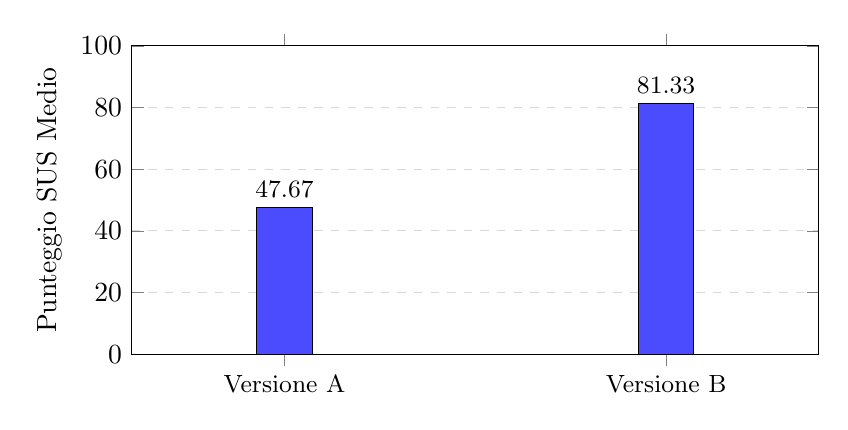
\begin{tikzpicture}
		\begin{axis}[
				ybar,
				bar width=20pt,
				width=0.85\textwidth,
				height=5.5cm,
				symbolic x coords={Versione A, Versione B},
				xtick=data,
				x tick label style={font=\small},
				ylabel={Punteggio SUS Medio},
				ymin=0, ymax=100,
				ymajorgrids=true,
				grid style={dashed, gray!30},
				enlarge x limits=0.4,
				nodes near coords,
				every node near coord/.style={font=\small, color=black, /pgf/number format/fixed, /pgf/number format/precision=2},
			]
			\addplot+[
				ybar,
				fill=blue!70,
				draw=black
			] coordinates {
					(Versione A,47.67)
					(Versione B,81.33)
				};
		\end{axis}
	\end{tikzpicture}
	\caption{Confronto generale dei punteggi medi SUS tra Versione A e Versione B.}
	\label{fig:6-sus-1}
\end{figure}

\paragraph{Confronto e analisi dell'effetto di ordine (A-B vs B-A)}
Scomponendo i dati in base alla sequenza di esecuzione, emergono variazioni rilevanti nella valutazione soggettiva che indicano la presenza di un forte effetto di contrasto legato all'ordine di esposizione dei prototipi.

Nel gruppo che ha affrontato la sequenza A-B (Figura~\ref{fig:6-sus-2}), valutando per prima la versione originale, i punteggi medi assegnati alla Versione A si sono attestati a 63,06. Sebbene si tratti di un valore ancora inferiore alla soglia di accettabilità, risulta sensibilmente più alto rispetto alla media globale, complici alcuni picchi di valutazione positiva (fino a 85,00) assegnati da utenti meno critici al primo impatto. Tuttavia, passando alla versione riprogettata, questo sotto-campione ha percepito immediatamente il netto miglioramento, assegnando alla Versione B una media eccellente pari a 89,44, con picchi che hanno sfiorato il punteggio massimo (97,50).

\begin{figure}[H]
	\centering
	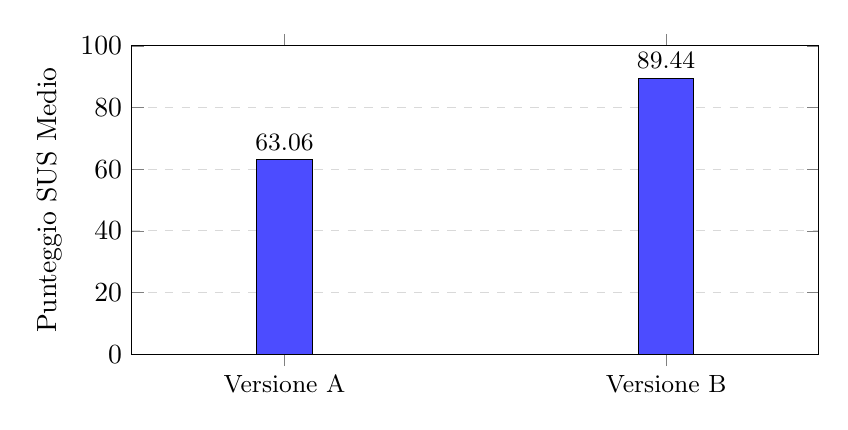
\begin{tikzpicture}
		\begin{axis}[
				ybar,
				bar width=20pt,
				width=0.85\textwidth,
				height=5.5cm,
				symbolic x coords={Versione A, Versione B},
				xtick=data,
				x tick label style={font=\small},
				ylabel={Punteggio SUS Medio},
				ymin=0, ymax=100,
				ymajorgrids=true,
				grid style={dashed, gray!30},
				enlarge x limits=0.4,
				nodes near coords,
				every node near coord/.style={font=\small, color=black, /pgf/number format/fixed, /pgf/number format/precision=2},
			]
			\addplot+[
				ybar,
				fill=blue!70,
				draw=black
			] coordinates {
					(Versione A,63.06)
					(Versione B,89.44)
				};
		\end{axis}
	\end{tikzpicture}
	\caption{Punteggi medi SUS relativi al sottogruppo con ordine di esecuzione A-B.}
	\label{fig:6-sus-2}
\end{figure}

Risultati nettamente differenti si osservano nel gruppo associato all'ordine B-A, come illustrato in Figura~\ref{fig:6-sus-3}. L'esperienza iniziale maturata sulla versione riprogettata (valutata con una media di 69,17) ha fissato un'aspettativa elevata riguardo alla linearità dei flussi e all'immediatezza dell'interfaccia. Di conseguenza, il successivo passaggio alla versione originale ha fortemente accentuato la percezione dei limiti strutturali, portando a una drastica e severa penalizzazione nei giudizi. In questa seconda sequenza, infatti, la Versione A ha registrato un crollo verticale, fermandosi a una media di appena 24,58, con valutazioni minime scese frequentemente tra 15,00 e 25,00.

\begin{figure}[H]
	\centering
	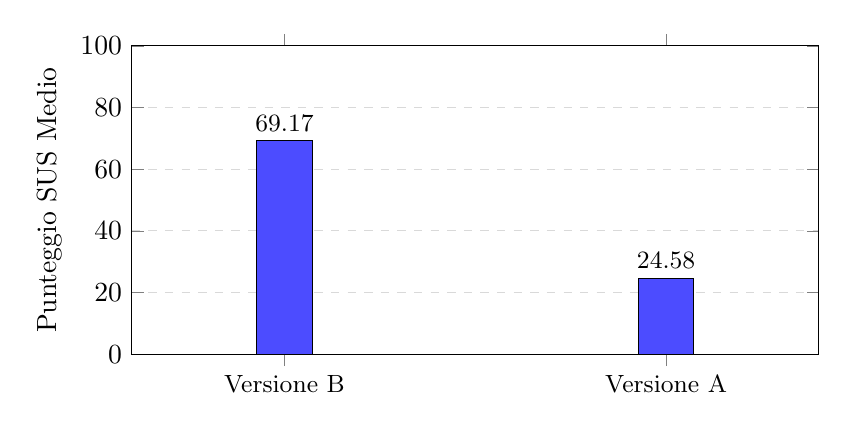
\begin{tikzpicture}
		\begin{axis}[
				ybar,
				bar width=20pt,
				width=0.85\textwidth,
				height=5.5cm,
				symbolic x coords={Versione B, Versione A},
				xtick=data,
				x tick label style={font=\small},
				ylabel={Punteggio SUS Medio},
				ymin=0, ymax=100,
				ymajorgrids=true,
				grid style={dashed, gray!30},
				enlarge x limits=0.4,
				nodes near coords,
				every node near coord/.style={font=\small, color=black, /pgf/number format/fixed, /pgf/number format/precision=2},
			]
			\addplot+[
				ybar,
				fill=blue!70,
				draw=black
			] coordinates {
					(Versione B,69.17)
					(Versione A,24.58)
				};
		\end{axis}
	\end{tikzpicture}
	\caption{Punteggi medi SUS relativi al sottogruppo con ordine di esecuzione B-A.}
	\label{fig:6-sus-3}
\end{figure}

Nonostante queste oscillazioni nei punteggi individuali introdotte dall'effetto di contrasto, la tendenza generale rimane inequivocabile: per la totalità del campione esaminato, indipendentemente dalla sequenza seguita, la Versione B ha ottenuto un punteggio SUS sistematicamente superiore rispetto alla Versione A, convalidando l'efficacia dell'intervento di riprogettazione.

Analizzando questi risultati emerge un'osservazione di particolare interesse per la valutazione della versione post-riprogettazione. Il punteggio SUS complessivo di 81,33 ottenuto dalla Versione B risente dell'effetto di contrasto sperimentato dal gruppo A–B. Considerando separatamente il gruppo B–A, che ha valutato la Versione B senza aver sperimentato in precedenza le criticità della versione originale, il punteggio medio risulta pari a 69,17. Sebbene tale valore superi la soglia convenzionalmente associata a una buona usabilità (68), esso suggerisce che la versione riprogettata presenti ancora margini di miglioramento quando viene valutata come sistema autonomo. Nel complesso, questi risultati indicano che parte della valutazione molto positiva osservata nel campione complessivo è attribuibile anche all'effetto di contrasto generato dal confronto diretto con la versione originale.
